% ============================================================================
%  EVNet Sentinel — IEEE research paper, v3 (7 pages)
%
%  Prepared for the mini-project research-paper submission. v2 stays the full
%  journal-track version and is not modified; v3 condenses it to 7 pages and
%  follows the required section structure:
%    Introduction, Literature Review, Proposed Methodology/Architecture
%    (3.1 Research Design, 3.2 Data, 3.3 Materials and Tools, 3.4 Procedure,
%    3.5 Data Analysis), Results, Discussion, Conclusion, Future Work,
%    References (>= 10, IEEE style).
%  Also reports flood F1 at four decimals instead of a rounded 1.000.
%
%  Build:    pdflatex EVNet_Sentinel_Research_Paper_v3.tex  (run twice)
% ============================================================================
\documentclass[conference]{IEEEtran}
\IEEEoverridecommandlockouts

\usepackage{cite}
\usepackage{amsmath,amssymb,amsfonts}
\usepackage{graphicx}
% figures/ is the Overleaf layout (zip upload); ../figures/ is this repository.
\graphicspath{{figures/}{../figures/}}
\usepackage{textcomp}
\usepackage{xcolor}
\usepackage{booktabs}
\usepackage{hyperref}
\usepackage{microtype}
\usepackage{tabularx}

\hypersetup{
    colorlinks=true, linkcolor=blue, urlcolor=blue, citecolor=blue,
    pdftitle={EVNet Sentinel: Leakage-Corrected Intrusion Detection for EV Charging Networks},
    pdfauthor={Varak, Chaurasiya, Chogale, Chavhan, Khandke}
}

\newcommand{\col}[1]{\texttt{\small #1}}
\newcolumntype{L}{>{\raggedright\arraybackslash}X}
\makeatletter
\newcommand{\linebreakand}{%
  \end{@IEEEauthorhalign}
  \hfill\mbox{}\par
  \mbox{}\hfill\begin{@IEEEauthorhalign}
}
\makeatother
\DeclareMathOperator*{\argmax}{arg\,max}

\begin{document}

\title{EVNet Sentinel: A Leakage-Corrected Reproduction and Comparative Study of Intrusion Detection on Electric Vehicle Charging Networks}

\author{
\IEEEauthorblockN{Mukta Varak}
\IEEEauthorblockA{\textit{Dept.\ of Computer Engineering} \\
\textit{Vidyalankar Institute of Technology}\\
Mumbai, India \\
24102A0013}
\and
\IEEEauthorblockN{Shruti Chaurasiya}
\IEEEauthorblockA{\textit{Dept.\ of Computer Engineering} \\
\textit{Vidyalankar Institute of Technology}\\
Mumbai, India \\
24102A0018}
\and
\IEEEauthorblockN{Shardul Chogale\textsuperscript{*}}
\IEEEauthorblockA{\textit{Dept.\ of Computer Engineering} \\
\textit{Vidyalankar Institute of Technology}\\
Mumbai, India \\
24102A0021}
\linebreakand
\IEEEauthorblockN{Neha Chavhan}
\IEEEauthorblockA{\textit{Dept.\ of Computer Engineering} \\
\textit{Vidyalankar Institute of Technology}\\
Mumbai, India \\
24102A0022}
\and
\IEEEauthorblockN{Mahesh Khandke}
\IEEEauthorblockA{\textit{Dept.\ of Computer Engineering} \\
\textit{Vidyalankar Institute of Technology}\\
Mumbai, India \\
makhandke@gmail.com}
\thanks{\textsuperscript{*}Corresponding author: Shardul Chogale (shardulchogale1983@gmail.com).}
}

\maketitle

% ============================================================================
\begin{abstract}
Public electric vehicle chargers are networked computers, and an attack on their link to the central management system can stop charging and billing. Machine-learning intrusion detectors evaluated on the CICEVSE2024 dataset report accuracies near 99 percent. This study reproduces the most recent of them, an online Adaptive Random Forest with ADWIN drift detection, and audits whether that accuracy reflects attack detection. We follow a quantitative, computational design: the published preprocessing is replayed, every feature is probed for label leakage, and four static classifiers and the online model are retrained on corrected data and evaluated over three seeds with macro-F1. A single capture timestamp recovers the attack label with 99.76 percent accuracy, above the published 98.40 percent, and the drift detector fires on the joins between capture files rather than on changes in traffic. After correction, flooding attacks remain near-perfectly separable while six network-scan types are not, and a mutual-information analysis shows that this limit lies in the flow features rather than in the models. A per-attack test finds that no attack passes as normal traffic and that Random Forest names attacks best with the fewest false alarms. The work is delivered as EVNet Sentinel, with a prediction service, role-based response guidance and an interactive web front end.
\end{abstract}

\begin{IEEEkeywords}
Intrusion detection, electric vehicle charging, CICEVSE2024, data leakage, adaptive random forest, concept drift, OCPP, machine learning evaluation
\end{IEEEkeywords}

% ============================================================================
\section{Introduction}

Electric mobility depends on a growing network of public charging stations (Electric Vehicle Supply Equipment, EVSE). Each station talks to the vehicle over ISO~15118 and to a Charging Station Management System (CSMS) over the Open Charge Point Protocol (OCPP) \cite{b14}. The OCPP link carries authorisation, metering and remote commands, so an attacker who floods or probes a station can interrupt charging and the revenue that depends on it \cite{b1,b3}. Detecting such attacks on the station network is therefore a practical security need.

Most detectors for this setting are machine-learning classifiers trained on the CICEVSE2024 dataset \cite{b8}, and reported accuracies are close to perfect \cite{b1,b2}. Makhmudov et al.\ \cite{b4} proposed the first online detector for charging networks, combining an Adaptive Random Forest (ARF) \cite{b6} with ADaptive WINdowing (ADWIN) \cite{b7} so the model can adapt as traffic changes, a problem known as concept drift \cite{b15}. They report 98.40\% multiclass accuracy.

Near-perfect scores on a public benchmark deserve scrutiny. Security datasets are often recorded one attack per capture, and features that identify the recording rather than the traffic can leak the label \cite{b10,b11,b13}. \textbf{The research problem} addressed here is whether the published accuracy measures attack detection or a property of how CICEVSE2024 was assembled. The problem is significant because an operator who trusts an inflated score will deploy a detector that fails on the attacks that matter.

\textbf{Objectives.} The study aims to (i) reproduce the published pipeline and test it for leakage; (ii) report corrected, multi-seed benchmarks of static and online models; (iii) explain which attacks remain hard and why; (iv) choose a primary detector per attack from detection, naming and false-alarm rates; and (v) deliver a usable system around the corrected models.

\textbf{Research questions.} The study is organised around four questions:
\begin{itemize}
    \item \textbf{RQ1:} Does the published preprocessing leak the label?
    \item \textbf{RQ2:} Is the reported drift real?
    \item \textbf{RQ3:} What accuracy remains once the leaks are removed, and which attacks are hard?
    \item \textbf{RQ4:} Which model should an operator trust, and for which attack?
\end{itemize}

\textbf{Contributions.} We present EVNet Sentinel, a passive network intrusion detection system for the station network, and use it to deliver five verifiable leakage findings, corrected benchmarks, a model-independent explanation of the reconnaissance ceiling, a per-attack evaluation with a confidence-gated naming rule, and a working prediction service and web front end.

% ============================================================================
\section{Literature Review}
\label{sec:lit}

\textbf{Surveys and threat analyses.} Bean et al.\ \cite{b1} survey machine-learning intrusion detection for charging equipment across network, host and power data and review 24 studies on CICEVSE2024; they identify concept drift and OCPP-level monitoring as open problems but take reported accuracies as given. Malimage et al.\ \cite{b3} analyse real incidents, protocol weaknesses (OCPP, OCPI) and standards such as ISO/SAE~21434, motivating detection without proposing a detector.

\textbf{Detectors on CICEVSE2024.} Joglekar et al.\ \cite{b2} combine a network detector (XGBoost, 99.99\% accuracy) with a host detector. They remove IP and MAC identifiers but keep timestamps, and train offline. Makhmudov et al.\ \cite{b4} stream the data through ARF+ADWIN with 20 trees and $\delta = 0.002$, reporting 99.13\% binary and 98.40\% multiclass accuracy, 11 drift events and 3.7\,ms per flow; drift handling is offered as the main advantage. Tanyildiz et al.\ \cite{b5} instead predict the time to the next attack with a GAN-augmented regressor on a different dataset.

\textbf{Online learning and drift.} Gama et al.\ \cite{b15} distinguish sudden, gradual and recurring drift and stress that a detector should be judged against the change it is meant to find. ARF \cite{b6} trains each tree with its own drift detector and replaces it with a background tree when drift is signalled. ADWIN \cite{b7} keeps a variable-length window of recent errors and cuts it when two sub-windows differ significantly. River \cite{b9} provides both. Random Forest \cite{b16}, the strongest static model in most flow-based studies, serves as the offline reference.

\textbf{Evaluation pitfalls.} Kaufman et al.\ \cite{b10} formalise leakage as information in the training data that would not be available at prediction time. Arp et al.\ \cite{b11} list sampling bias, spurious correlations and inappropriate baselines among the most common errors in security machine learning, and Sommer and Paxson \cite{b13} warn that intrusion detectors often learn artefacts of the evaluation environment.

\begin{table}[!t]
\caption{Comparison of related work with this study}
\label{tab:comparison}
\centering
\footnotesize
\begin{tabularx}{\columnwidth}{@{}lLLc@{}}
\toprule
\textbf{Work} & \textbf{Approach} & \textbf{Reported} & \textbf{Audit} \\
\midrule
Bean \cite{b1} & Survey (24 studies) & --- & $\times$ \\
Joglekar \cite{b2} & XGBoost + host IDS, offline & 99.99\% acc. & IP/MAC \\
Malimage \cite{b3} & Threat analysis & --- & --- \\
Makhmudov \cite{b4} & ARF+ADWIN, online & 98.40\% acc. & $\times$ \\
Tanyildiz \cite{b5} & GAN time-to-attack & $R^2 = 0.74$ & --- \\
\midrule
\textbf{This work} & \textbf{Audit + 4 models + ARF, 3 seeds} & \textbf{0.558 macro-F1} & \checkmark \\
\bottomrule
\end{tabularx}
\end{table}

\textbf{Research gap.} Table~\ref{tab:comparison} shows that no prior CICEVSE2024 study tests its preprocessing for capture-level leakage, reports results over several seeds, uses a class-balanced metric as the headline, or checks whether detected drift is real. This study addresses all four gaps and adds a per-attack, operator-oriented evaluation.

% ============================================================================
\section{Proposed Methodology and Architecture}
\label{sec:method}

Fig.~\ref{fig:pipeline} summarises the method and the delivered system, from capture to response.

\begin{figure*}[!t]
\centering
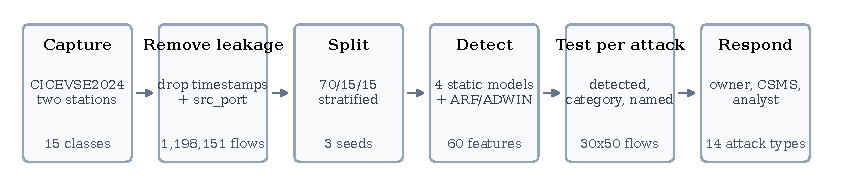
\includegraphics[width=\textwidth]{fig_pipeline.pdf}
\caption{Method and system at a glance, from capture to response.}
\label{fig:pipeline}
\end{figure*}

\subsection{Research Design}

The study is \emph{quantitative and computational}, in two parts. The first is a \emph{reproduction audit}: the published pipeline is replayed exactly and each suspected artefact is isolated with a controlled experiment that changes one factor at a time (a feature, the stream order, or the split). The second is a \emph{comparative experiment}: four static classifiers and the online model are trained on corrected data under one protocol. This design suits the objectives because each finding becomes a measurable, repeatable test rather than an opinion, and every number can be regenerated from the public code.

The detector is \emph{passive}. It reads a mirrored copy of the switch traffic, classifies each completed network flow and raises an alert, but never blocks traffic. This matches how CICEVSE2024 itself was recorded.

\subsection{Data}

CICEVSE2024 \cite{b8} was recorded by the Canadian Institute for Cybersecurity on a testbed with two charging stations (EVSE-A and EVSE-B), a local and a remote CSMS, and a vehicle controller, with stations either idle or charging. Network flows were extracted with NFStream into 86 features and labelled from the capture file name. The 59 capture files hold 2,744,700 flows in 15 classes:
\begin{itemize}
    \item five \emph{volumetric floods}: SYN, TCP, UDP, PSH-ACK and SynonymousIP;
    \item six \emph{nmap reconnaissance modes}: TCP port scan, SYN stealth scan, OS fingerprinting, service-version detection, vulnerability scan and aggressive scan;
    \item three \emph{low-rate attacks}: ICMP flood, ICMP fragmentation and Slowloris;
    \item benign traffic.
\end{itemize}

The dataset lists its devices but not which device attacked which. Because every flow carries source and destination MAC addresses, we derived the route of each attack capture (Table~\ref{tab:routes}). Every attack targets a charging station, and in six captures the compromised vehicle scans EVSE-B over the charging cable.

\begin{table}[!t]
\caption{Attack routes derived from MAC addresses (57 attack captures)}
\label{tab:routes}
\centering
\footnotesize
\begin{tabularx}{\columnwidth}{@{}llrL@{}}
\toprule
\textbf{Attacker} & \textbf{Target} & \textbf{Caps.} & \textbf{Attacks} \\
\midrule
Kali PC (Wi-Fi)       & EVSE-A & 24 & all except UDP flood \\
Kali PC (Wi-Fi)       & EVSE-B & 23 & all except UDP flood, Slowloris \\
Raspberry Pi (Wi-Fi)  & both   & 4  & UDP flood \\
Compromised vehicle   & EVSE-B & 6  & the six scans \\
\bottomrule
\end{tabularx}
\end{table}

The classes are highly imbalanced: after deduplication the four large floods hold about 196,000--260,000 flows each, the scans 28,000--39,000, Slowloris 2,721, and benign traffic only 81.

\subsection{Materials and Tools}

All experiments ran on one Apple M5 laptop (10 cores, 16\,GB RAM) with pinned software versions:
\begin{itemize}
    \item \textbf{Analysis:} Python 3.13, NumPy 2.4, pandas and scikit-learn 1.8 \cite{b12} for the static models, and River 0.26 \cite{b9} for ARF+ADWIN.
    \item \textbf{Service:} a FastAPI prediction service that loads every model and its scaler at start-up.
    \item \textbf{Front end:} a Next.js 16 web application.
    \item \textbf{Reporting:} matplotlib for every figure, drawn from the same exported data the front end displays.
\end{itemize}
The dataset, code and exported results are public (Section~\ref{sec:conclusion}).

\subsection{Procedure}

\textbf{Step 1, replay.} The reference preprocessing \cite{b4} was rerun verbatim to reproduce its feature set.

\textbf{Step 2, leakage probes.} A depth-25 decision tree was trained on each feature alone and scored by 3-fold cross-validated accuracy. Keeping or dropping each suspicious column was crossed before deduplication.

\textbf{Step 3, corrected preprocessing.} All captures are concatenated and labelled. Identifiers (flow ID, IP, MAC, vendor) and constant columns are removed. The six absolute timestamps (\col{*\_first\_seen\_ms}, \col{*\_last\_seen\_ms}) and \col{src\_port} are dropped, while the destination port is kept. Duplicate rows are removed, the data are split 70/15/15 with class stratification, and each feature is standardised with training statistics only. This leaves 1,198,151 flows and 60 features (838,705 / 179,723 / 179,723 rows).

\textbf{Step 4, training.} The static models are:
\begin{itemize}
    \item Random Forest \cite{b16}: 100 trees, depth 15;
    \item Decision Tree: depth 20;
    \item Logistic Regression and a linear SVM, both trained by stochastic gradient descent.
\end{itemize}
All four use balanced class weights $w_k = N/(K n_k)$, so that rare classes count as much as common ones. ARF uses the published configuration: 20 trees, half the features per split, a grace period of 30, and ADWIN with $\delta = 0.002$. It is run prequentially, predicting each flow before learning from it, in both capture order and shuffled order.

\textbf{Step 5, per-attack testing.} For each attack, model and seed, 30 batches of 50 unseen flows are scored. Mixed campaigns of four simultaneous attacks are also run. Regression gates fail the run if detection of any attack falls below 0.95.

\textbf{Step 6, delivery.} The models are served by the API, and the exported results drive the web dashboard and a simulation that replays held-out flows along their recorded routes.

\subsection{Data Analysis}

\textbf{Metrics.} For class $k$ with precision $P_k$ and recall $R_k$,
\begin{equation}
F_{1,k} = \frac{2 P_k R_k}{P_k + R_k}, \qquad
\text{macro-}F_1 = \frac{1}{K} \sum_{k=1}^{K} F_{1,k}.
\label{eq:f1}
\end{equation}
Macro-$F_1$ weights the 15 classes equally. Accuracy, by contrast, is dominated by the floods. Every figure is the mean and standard deviation over seeds 42, 1337 and 2024, where each seed changes both the split and the model initialisation.

\textbf{Stream order.} Prequential accuracy is compared with the trivial rule ``repeat the previous label''. That rule's accuracy equals the label autocorrelation
\begin{equation}
\rho = \Pr\left[y_t = y_{t-1}\right],
\label{eq:rho}
\end{equation}
which any model on an ordered stream must beat before it can be said to learn. For a shuffled stream $\rho = \sum_k p_k^2$, where $p_k$ is the share of class $k$.

\textbf{ADWIN.} ADWIN signals drift when, for some split of its window $W$ into $W_0 W_1$, the mean error of the two parts differs by more than
\begin{equation}
\epsilon_{\text{cut}} = \sqrt{\frac{1}{2m}\ln\frac{4n}{\delta}}, \qquad m = \frac{1}{1/n_0 + 1/n_1},
\label{eq:adwin}
\end{equation}
where $n_0$ and $n_1$ are the sizes of the two parts and $n = |W|$. In capture order every file boundary is an abrupt change by construction, so we test whether the alarms fall on them.

\textbf{Drift alignment.} For each ADWIN alarm $e_i$, we measure the distance to the nearest capture-file boundary, $d_i = \min_j |e_i - b_j|$. We count the alarms within $w = 100$ flows of a boundary and compare that count $H$ with the counts $H^{(r)}$ from $R = 2000$ random placements of the same number of alarms:
\begin{equation}
p = \frac{1 + \sum_{r=1}^{R}\mathbb{I}\left[H^{(r)} \ge H\right]}{1 + R}.
\label{eq:pvalue}
\end{equation}

\textbf{Per-feature separability.} Within one category $g$ (DoS or reconnaissance), we measure how much of the class uncertainty a single feature $X_j$ removes:
\begin{equation}
S_j^{(g)} = \frac{I\left(X_j;\,Y \mid g\right)}{H\left(Y \mid g\right)},
\label{eq:sep}
\end{equation}
estimated with a $k$-nearest-neighbour mutual-information estimator \cite{b17} on 6,000 held-out flows per category. $S_j$ does not depend on any model, so it describes the data itself.

\textbf{Per-attack rates.} For each batch we measure three rates: the share detected (called any attack), the share placed in the right category, and the share named exactly. On benign flows we measure the false-alarm rate. The primary detector is the model with the fewest false alarms among those whose mean exact-naming rate is within 0.02 of the best.

\textbf{Confidence gating.} A model names an attack only if its top class probability is at least $t$:
\begin{equation}
\text{output}(\mathbf{x}) =
\begin{cases}
\argmax_k \hat{p}(k\mid\mathbf{x}) & \text{if } \max_k \hat{p}(k\mid\mathbf{x}) \ge t,\\
\text{category of that class} & \text{otherwise.}
\end{cases}
\label{eq:gate}
\end{equation}

% ============================================================================
\section{Results}
\label{sec:results}

\subsection{Leakage in the published pipeline}

Table~\ref{tab:leak} lists the leakage probes. A decision tree on \col{bidirectional\_first\_seen\_ms} alone recovers the 15-class label with 0.9976 accuracy, above the 0.9840 reported for the full published model. The reference preprocessing keeps all six timestamp columns. It also drops \col{dst\_port}, the feature that defines a port scan. The source port, which the operating system allocates almost sequentially, alone recovers 0.4028.

Table~\ref{tab:ablation} shows why the published configuration is fragile. Dropping the destination port while keeping the timestamps leaves 273,932 reconnaissance flows after deduplication. These flows can then be separated by \emph{when} they were captured rather than by what they did. Removing both the timestamps and the destination port collapses the scans to 6,821 flows: almost every remaining scan flow becomes a duplicate.

\begin{table}[!t]
\caption{Flows left after deduplication, by kept or dropped column}
\label{tab:ablation}
\centering
\footnotesize
\begin{tabular}{@{}llrr@{}}
\toprule
\textbf{Timestamps} & \textbf{\col{dst\_port}} & \textbf{Total} & \textbf{Recon.} \\
\midrule
kept & kept & 2,728,799 & 1,724,504 \\
\textbf{kept} & \textbf{dropped (published)} & \textbf{1,277,520} & \textbf{273,932} \\
dropped & kept (ours) & 1,198,143 & 194,737 \\
dropped & dropped & 977,862 & 6,821 \\
\bottomrule
\end{tabular}
\end{table}

\begin{table}[!t]
\caption{Label recovered from a single feature (15 classes, 3-fold CV)}
\label{tab:leak}
\centering
\footnotesize
\begin{tabular}{@{}llr@{}}
\toprule
\textbf{Feature} & \textbf{Nature} & \textbf{Accuracy} \\
\midrule
\col{bidirectional\_first\_seen\_ms} & fingerprint & \textbf{0.9976} \\
\col{src\_port} & partial & 0.4028 \\
\col{dst\_port} & legitimate & 0.2917 \\
\midrule
\multicolumn{2}{@{}l}{\emph{Published multiclass accuracy \cite{b4}}} & \emph{0.9840} \\
\bottomrule
\end{tabular}
\end{table}

\subsection{Stream order and drift}

In capture order each file holds a single class, so over 1,921,182 training flows the label changes only 54 times and $\rho = 0.99997$ (Table~\ref{tab:order}). ARF+ADWIN reaches 0.9997, which does not beat the repeat-last rule. On a shuffled stream it reaches 0.5585.

\begin{table}[!t]
\caption{ARF+ADWIN prequential accuracy by stream order (leak-free)}
\label{tab:order}
\centering
\footnotesize
\begin{tabular}{@{}lrrr@{}}
\toprule
\textbf{Order} & \textbf{ARF acc.} & \textbf{Repeat-last $\rho$} & \textbf{Drift alarms} \\
\midrule
Capture order & 0.9997 & 0.99997 & 43 \\
Shuffled & 0.5585 & 0.117 & 14 \\
\bottomrule
\end{tabular}
\end{table}

Of the 43 drift alarms in capture order, 42 lie within 100 flows of a file boundary, with a median distance of 22 flows. Random placement would put only $2.2 \pm 1.5$ alarms that close ($p < 0.0005$), as Fig.~\ref{fig:drift} shows.

\begin{figure}[!t]
\centering
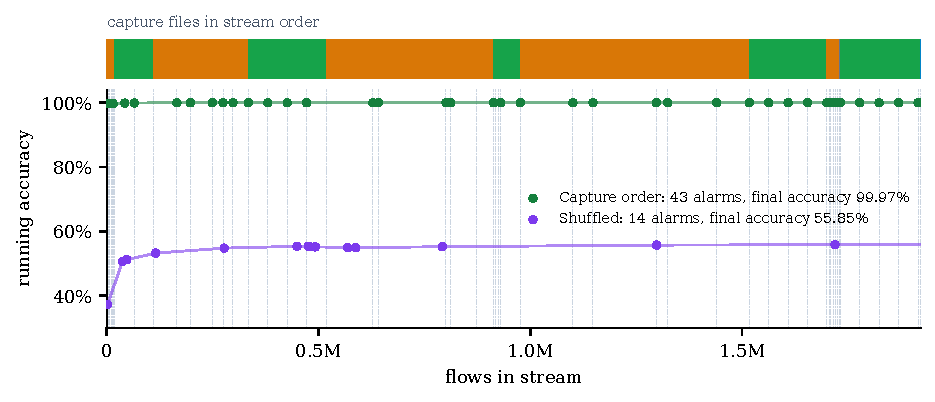
\includegraphics[width=\columnwidth]{fig_drift.pdf}
\caption{ADWIN alarms over the training stream. Top band: the 58 capture files in stream order. Dashed lines mark file boundaries.}
\label{fig:drift}
\end{figure}

\subsection{Corrected benchmarks}

Table~\ref{tab:results} gives the corrected results. Random Forest and Decision Tree are within one standard deviation of each other, the linear models trail by more than 0.1 macro-$F_1$, and all four reach about 0.86 accuracy. On a like-for-like split, removing the timestamps lowers Random Forest's macro-$F_1$ from 0.9547 to 0.5894, while the SVM changes by only $+0.03$. Removing \col{src\_port}, with the rows and the split held fixed, costs the deeper Decision Tree twice as much as Random Forest (Table~\ref{tab:srcport}). Extra depth was buying finer bands of port numbers, so the tree's earlier advantage was memorisation.

\begin{table}[!t]
\caption{Effect of removing \col{src\_port} (macro-$F_1$, single seed)}
\label{tab:srcport}
\centering
\footnotesize
\begin{tabular}{@{}lrrr@{}}
\toprule
\textbf{Model} & \textbf{With} & \textbf{Without} & \textbf{$\Delta$} \\
\midrule
Random Forest & 0.5894 & 0.5138 & $-0.076$ \\
Decision Tree & 0.6834 & 0.5135 & $\mathbf{-0.170}$ \\
\bottomrule
\end{tabular}
\end{table}

\begin{table}[!t]
\caption{Multiclass results, mean $\pm$ std over 3 seeds (corrected features)}
\label{tab:results}
\centering
\footnotesize
\begin{tabular}{@{}lrrr@{}}
\toprule
\textbf{Model} & \textbf{Macro-$F_1$} & \textbf{Acc.} & \textbf{Fit (s)} \\
\midrule
Random Forest & \textbf{0.558$\pm$0.008} & 0.868 & 8.5 \\
Decision Tree & 0.557$\pm$0.010 & 0.868 & 3.4 \\
Logistic Regression & 0.436$\pm$0.017 & 0.863 & 78.9 \\
Linear SVM & 0.411$\pm$0.017 & 0.862 & 34.9 \\
\bottomrule
\end{tabular}
\end{table}

\subsection{Per-class results and separability}

Table~\ref{tab:perclass} shows a sharp split. The five floods reach $F_1 \ge 0.999$ in every seed. The six scans average 0.183, and sample size does not explain the gap: UDP flood (32,072 flows) scores 0.9994, while TCP port scan (35,123 flows) scores 0.265. The separability measure (Fig.~\ref{fig:separability}) shows the same split. Within DoS, one inter-arrival-time feature resolves 98\% of the class uncertainty. Within reconnaissance, the best feature resolves 5\%.

The errors among the scans follow a pattern (Fig.~\ref{fig:confusion}). Random Forest labels 32--48\% of every other scan as OS fingerprinting, so the scans collapse into one ``sink'' class. A further 8--11\% of each scan is labelled Slowloris, because both hold long-lived, nearly idle connections. This confusion accounts for almost all of the error between the reconnaissance and DoS categories.

\begin{figure}[!t]
\centering
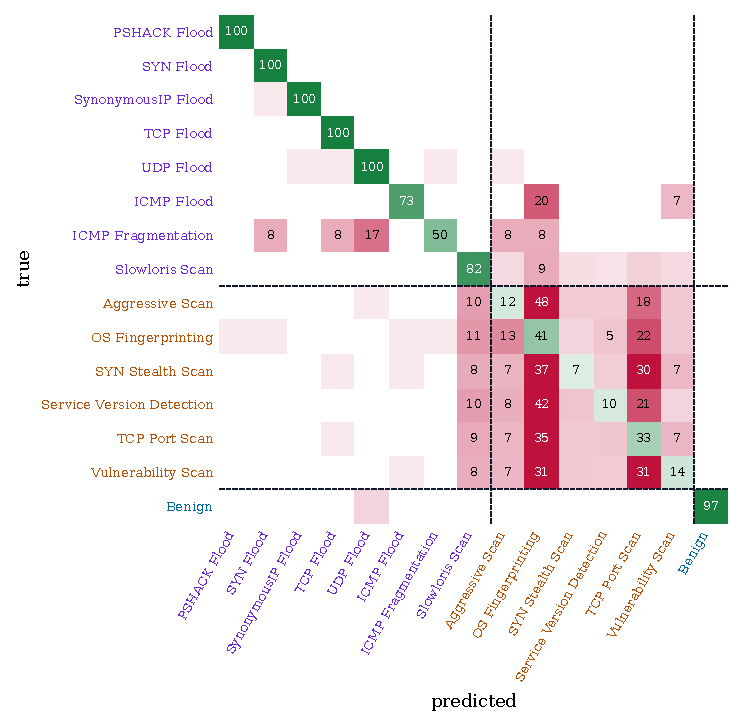
\includegraphics[width=\columnwidth]{fig_confusion_rf.pdf}
\caption{Random Forest confusion matrix, row-normalised and averaged over three seeds (\%; cells under 5\% unlabelled). Dashed lines separate DoS, reconnaissance and benign.}
\label{fig:confusion}
\end{figure}

\begin{table}[!t]
\caption{Per-class $F_1$, Random Forest, mean $\pm$ std over 3 seeds}
\label{tab:perclass}
\centering
\footnotesize
\begin{tabular}{@{}lrr@{}}
\toprule
\textbf{Class} & \textbf{Support} & \textbf{$F_1$} \\
\midrule
SYN, TCP, PSH-ACK, SynIP & 196k--259k & 0.9999$\pm$0.0000 \\
UDP flood & 32,072 & 0.9994$\pm$0.0001 \\
\midrule
TCP port scan & 35,123 & 0.265 \\
OS fingerprinting & 27,702 & 0.223 \\
Vulnerability scan & 39,002 & 0.204 \\
Service-version detection & 30,338 & 0.156 \\
Aggressive scan & 27,815 & 0.145 \\
SYN stealth scan & 34,765 & 0.105 \\
\midrule
Benign & 81 & 0.986 \\
ICMP flood / ICMP fragmentation & 32 / 28 & 0.660 / 0.439 \\
Slowloris & 2,721 & 0.191 \\
\bottomrule
\end{tabular}
\end{table}

\begin{figure*}[!t]
\centering
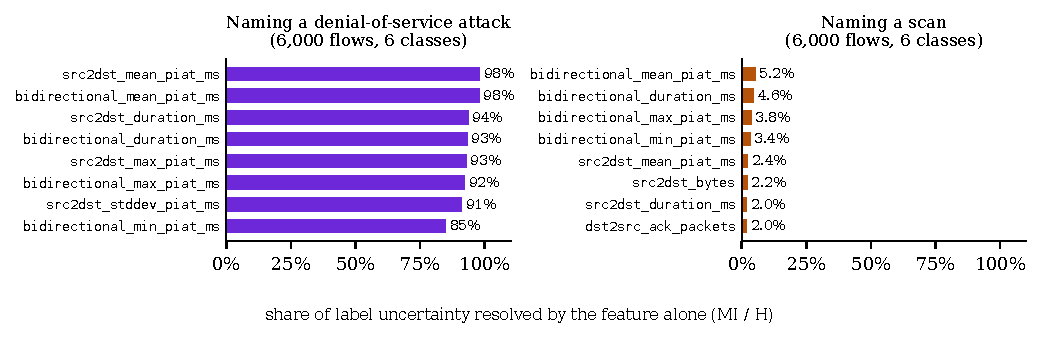
\includegraphics[width=0.82\textwidth]{fig_separability.pdf}
\caption{Per-feature separability $S_j$ of \eqref{eq:sep} within DoS and within reconnaissance flows (6,000 held-out flows each).}
\label{fig:separability}
\end{figure*}

\subsection{Per-attack detection and confidence}

Table~\ref{tab:perattack} lists the exact-naming rate per attack. Across 90 mixed campaigns, every model flags at least 99.9\% of attack flows as malicious. Every model names the floods exactly ($\ge 0.98$). The scans are placed in the right category 96\% of the time by the best model for each, but named exactly only 34\% of the time. Table~\ref{tab:fa} gives the false-alarm rates on benign traffic. By the selection rule of Section~\ref{sec:method}, Random Forest is the primary detector. Applying the confidence gate \eqref{eq:gate} at $t = 0.5$ cuts Random Forest's wrong scan names from 81\% to 3\% and reports 94\% of scans by category, while 93\% of DoS flows are still named exactly (Table~\ref{tab:gate}).

\begin{table}[!t]
\caption{Exact-naming rate $E$ per attack for Random Forest, the best model at naming, and the best category rate $C$}
\label{tab:perattack}
\centering
\footnotesize
\begin{tabular}{@{}lrlr@{}}
\toprule
\textbf{Attack} & \textbf{RF $E$} & \textbf{Best $E$} & \textbf{Best $C$} \\
\midrule
Five volumetric floods & 1.00 & all ($\ge 0.98$) & 1.00 \\
Slowloris & 0.82 & RF & 0.82 \\
TCP port scan & 0.32 & LR 0.65 & 0.97 \\
OS fingerprinting & 0.41 & RF/DT 0.41 & 0.95 \\
SYN stealth scan & 0.06 & SVM 0.43 & 0.97 \\
Vulnerability scan & 0.13 & SVM 0.26 & 0.97 \\
Aggressive scan & 0.12 & DT 0.15 & 0.94 \\
Service-version det. & 0.10 & DT 0.13 & 0.96 \\
\bottomrule
\end{tabular}
\end{table}

\begin{table}[!t]
\caption{Confidence-gated naming for Random Forest: share named right ($R$), named wrong ($W$), reported by category only ($H$)}
\label{tab:gate}
\centering
\footnotesize
\begin{tabular}{@{}lrrrrrr@{}}
\toprule
 & \multicolumn{3}{c}{\textbf{DoS}} & \multicolumn{3}{c}{\textbf{Reconnaissance}} \\
\cmidrule(lr){2-4}\cmidrule(lr){5-7}
$t$ & $R$ & $W$ & $H$ & $R$ & $W$ & $H$ \\
\midrule
0   & 0.97 & 0.03 & 0.00 & 0.19 & 0.81 & 0.00 \\
0.5 & 0.93 & 0.00 & 0.07 & 0.03 & 0.03 & 0.94 \\
0.9 & 0.87 & 0.00 & 0.13 & 0.01 & 0.00 & 0.99 \\
\bottomrule
\end{tabular}
\end{table}

\begin{table}[!t]
\caption{False-alarm rate on benign traffic by model}
\label{tab:fa}
\centering
\footnotesize
\begin{tabular}{@{}lrrrr@{}}
\toprule
 & \textbf{RF} & \textbf{DT} & \textbf{LR} & \textbf{SVM} \\
\midrule
False-alarm rate & \textbf{0.02} & 0.12 & 0.46 & 0.59 \\
\bottomrule
\end{tabular}
\end{table}

% ============================================================================
\section{Discussion}
\label{sec:discussion}

\textbf{What the published accuracy measures.} Each attack was recorded in its own file at its own time, so an absolute timestamp identifies the recording, and through it the label. This is leakage in the sense of Kaufman et al.\ \cite{b10}: the feature would not carry this information on live traffic. Trees exploit it and linear models cannot, which is why removing the timestamps costs Random Forest 0.365 macro-$F_1$ but leaves the SVM almost unchanged. Much of the reported gap between tree and linear models in earlier work therefore reflects how well each model could use the leak.

\textbf{Drift.} The online model's capture-order accuracy equals the repeat-last baseline, and its drift alarms coincide with file boundaries. Both observations point the same way: the stream changes where files were joined, not because charging traffic evolved. Drift handling is presented in \cite{b4} as the method's advantage, but CICEVSE2024 contains no real drift with which to test that claim. This matches the warnings of Arp et al.\ \cite{b11} about inappropriate baselines and of Sommer and Paxson \cite{b13} about learning artefacts of the evaluation environment.

\textbf{Floods and scans.} The near-perfect flood scores are plausible rather than leaked. The fingerprint columns are removed; a flood has a strong physical signature that a single timing feature captures; and the linear models also name the floods. We nevertheless claim this only for this testbed: the random split can place near-identical flows from one capture on both sides of the split, and floods sent at a lower rate would look different. The scans are a different matter. All six are modes of one tool, the aggressive mode includes two of the others, and Fig.~\ref{fig:separability} shows that no single flow statistic separates them. More model capacity cannot recover information the features do not contain.

\textbf{Operational meaning.} No attack passes as normal traffic. The weakness is \emph{naming}, not \emph{noticing}. Random Forest names attacks as well as any model and raises the fewest false alarms, so it is the primary detector. For scans, a confidence gate turns confidently wrong names into correct category alerts, which is the information an operator can act on.

\textbf{Limitations.} Labels come from file names, so background traffic recorded during an attack carries the attack's label. Only 81 benign flows exist, so false-alarm rates are indicative. The headline results use a random rather than a grouped split. The study covers a single testbed with tools at default settings, and the host and power data in CICEVSE2024 are not used.

% ============================================================================
\section{Conclusion}
\label{sec:conclusion}

This study set out to test whether the high accuracies reported on CICEVSE2024 measure attack detection, and found that they largely do not:
\begin{itemize}
    \item one capture timestamp beats the published model;
    \item streaming accuracy in capture order is matched by repeating the previous label;
    \item the drift detector responds to file boundaries.
\end{itemize}
With these effects removed, the corrected benchmark is 0.558 macro-$F_1$ for Random Forest over three seeds. Volumetric floods remain near-perfectly separable on this testbed, while the six nmap scan modes are not, and a model-independent analysis places that limit in the flow features. Operationally, every attack is detected, Random Forest is the recommended detector, and requiring confidence before naming an attack replaces most wrong scan names with correct category alerts. The system, code and results are public at \url{https://github.com/Mukta01/EVNet_Sentinel}.

% ============================================================================
\section{Future Work and Recommendations}

\begin{enumerate}
    \item \textbf{Grouped evaluation.} Report results with whole capture files held out, which removes near-duplicate flows from both sides of the split.
    \item \textbf{Sequence features.} Model the packet sequence within each flow, which flow statistics discard and which may separate the scan modes.
    \item \textbf{More modalities.} Fuse the host-event and power traces in CICEVSE2024 with the network flows.
    \item \textbf{Stronger baselines for online learning.} Evaluate every streaming model against the repeat-last rule \eqref{eq:rho} on grouped streams.
    \item \textbf{Response.} Measure the response guidance itself, for example a quarantine of the attacking device approved by an operator, on a live testbed.
    \item \textbf{Recommendation for dataset builders.} Release per-capture identifiers and benign traffic in volume, so that leakage can be checked and false alarms measured.
\end{enumerate}

\section*{Acknowledgment}

We build on the open-source implementation of \cite{b4} and thank the Canadian Institute for Cybersecurity for the CICEVSE2024 dataset.

% ============================================================================
\begin{thebibliography}{00}

\bibitem{b1} J.\ Bean, V.\ Manias et al., ``Cybersecurity of electric vehicle charging infrastructure: Recent advances, open challenges, and future directions,'' arXiv:2605.24190v1, May 2026.

\bibitem{b2} C.\ Joglekar et al., ``A hybrid intrusion detection system for electric vehicle charging infrastructure,'' arXiv:2606.23236v1, 2026.

\bibitem{b3} K.\ Malimage et al., ``Cybersecurity challenges in the electric vehicle market,'' in \emph{Proc.\ CIGRE Canada Conf.}, 2023, pp.\ 1--6.

\bibitem{b4} F.\ Makhmudov, D.\ Kilichev, U.\ Giyosov, and F.\ Akhmedov, ``Online machine learning for intrusion detection in electric vehicle charging systems,'' \emph{Mathematics}, vol.\ 13, no.\ 5, p.\ 712, 2025, doi: 10.3390/math13050712.

\bibitem{b5} E.\ Tanyildiz et al., ``Detection of cyber attacks in electric vehicle charging systems using a remaining useful life generative adversarial network,'' \emph{Scientific Reports}, vol.\ 15, 2025.

\bibitem{b6} H.\ M.\ Gomes et al., ``Adaptive random forests for evolving data stream classification,'' \emph{Machine Learning}, vol.\ 106, no.\ 9--10, pp.\ 1469--1495, 2017.

\bibitem{b7} A.\ Bifet and R.\ Gavald\`{a}, ``Learning from time-changing data with adaptive windowing,'' in \emph{Proc.\ SIAM Int.\ Conf.\ Data Mining}, 2007, pp.\ 443--448.

\bibitem{b8} Canadian Institute for Cybersecurity, ``CICEVSE2024 dataset,'' University of New Brunswick, 2024. [Online]. Available: \url{https://www.unb.ca/cic/datasets/}

\bibitem{b9} J.\ Montiel et al., ``River: Machine learning for streaming data in Python,'' \emph{J.\ Mach.\ Learn.\ Res.}, vol.\ 22, no.\ 110, pp.\ 1--8, 2021.

\bibitem{b10} S.\ Kaufman, S.\ Rosset, C.\ Perlich, and O.\ Stitelman, ``Leakage in data mining: Formulation, detection, and avoidance,'' \emph{ACM Trans.\ Knowl.\ Discov.\ Data}, vol.\ 6, no.\ 4, pp.\ 1--21, 2012.

\bibitem{b11} D.\ Arp et al., ``Dos and don'ts of machine learning in computer security,'' in \emph{Proc.\ 31st USENIX Security Symp.}, 2022, pp.\ 3971--3988.

\bibitem{b12} F.\ Pedregosa et al., ``Scikit-learn: Machine learning in Python,'' \emph{J.\ Mach.\ Learn.\ Res.}, vol.\ 12, pp.\ 2825--2830, 2011.

\bibitem{b13} R.\ Sommer and V.\ Paxson, ``Outside the closed world: On using machine learning for network intrusion detection,'' in \emph{Proc.\ IEEE Symp.\ Security and Privacy}, 2010, pp.\ 305--316.

\bibitem{b14} Open Charge Alliance, ``Open Charge Point Protocol 2.0.1,'' 2020. [Online]. Available: \url{https://openchargealliance.org/protocols/open-charge-point-protocol/}

\bibitem{b15} J.\ Gama, I.\ \v{Z}liobait\.{e}, A.\ Bifet, M.\ Pechenizkiy, and A.\ Bouchachia, ``A survey on concept drift adaptation,'' \emph{ACM Comput.\ Surv.}, vol.\ 46, no.\ 4, pp.\ 1--37, 2014.

\bibitem{b16} L.\ Breiman, ``Random forests,'' \emph{Machine Learning}, vol.\ 45, no.\ 1, pp.\ 5--32, 2001.

\bibitem{b17} A.\ Kraskov, H.\ St\"{o}gbauer, and P.\ Grassberger, ``Estimating mutual information,'' \emph{Physical Review E}, vol.\ 69, no.\ 6, p.\ 066138, 2004.

\end{thebibliography}

\end{document}
